%%%%%%%%%%%%%%%%%%%%% {{{
%%Options for presentations (in-class) and handouts (e.g. print).
\documentclass[pdf,9pt]{beamer}
% \documentclass[pdf,9pt]{beamer}


%%%%%%%%%%%%%%%%%%%%%%
%Change this for different slides so it appears in bar
\usepackage{authoraftertitle}
\date{Chapter 2. Matrix Algebra \\ \S 2-7. LU Factorization}

%%%%%%%%%%%%%%%%%%%%%%
%% Upload common style file
\usepackage{LyryxLAWASlidesStyle}

\begin{document}

%%%%%%%%%%%%%%%%%%%%%%%
%% Title Page and Copyright Common to All Slides

%Title Page
\input frontmatter/titlepage.tex

%LOTS Page
\input frontmatter/lyryxopentexts.tex

%Copyright Page
\input frontmatter/copyright.tex

%%%%%%%%%%%%%%%%%%%%%%%%% }}}

%-------------- start slide -------------------------------%{{{ 2
\begin{frame}[fragile]
   \tableofcontents
\end{frame}
%-------------- end slide -------------------------------%}}}

\section[\textcolor{yellow}{}]{\textcolor{yellow}{LU Factorization}}

%-------------- start slide -------------------------------%{{{ 3
\frame{
\frametitle{LU Factorization}
\pause
\begin{definition}
    A matrix $A = \leftB a_{ij} \rightB$ is called \alert{upper triangular} if $a_{ij} = 0$ whenever $i > j$. Thus the entries below the main diagonal equal $0$.

    \pause
    \begin{center}
	    
\begin{tikzpicture}[scale=1, transform shape]
	    \tikzset{>=latex}
	    \filldraw[color=teal] (0,1) -- (1,1) -- (1,0);
	    \filldraw[color=teal] (1.5,1) -- (2,1) -- (2,0.5);
	    \filldraw[color=teal] (2.5,1) -- (4,1) -- (4,0) -- (3.5,0);
	    \draw[color=yellow,thick] (0,0) rectangle (1,1);
	    \draw[color=yellow,thick] (1.5,0) rectangle (2,1);
	    \draw[color=yellow,thick] (2.5,0) rectangle (4,1);
	    \node[] (0) at (0.3,0.3) {$0$};
	    \node[] (0) at (1.75,0.3) {$0$};
	    \node[] (0) at (2.8,0.3) {$0$};
	    \end{tikzpicture}
    \end{center}
    % \begin{align*}
    % \leftB
    % \begin{array}{cccc}
    % * & * & \cdots & * \\
    % 0 & * & \cdots & \vdots \\
    % \vdots & \vdots & \ddots & * \\
    % 0 & \cdots & 0 & *
    % \end{array}
    % \rightB,
    % \quad
    % \leftB
    % \begin{array}{cccc}
    % * & * & \cdots & * \\
    % 0 & * & \cdots & \vdots \\
    % \vdots & \vdots & \ddots & * \\
    % 0 & \cdots & 0 & * \\
    % 0 & \cdots & 0 & 0
    % \end{array}
    % \rightB
    % \end{align*}
    % where $*$ refers to any number.
    \pause
    A  \alert{lower triangular matrix} is defined similarly, as a matrix for which all entries \textbf{above} the main diagonal are equal to zero.
    \pause
    \begin{center}
	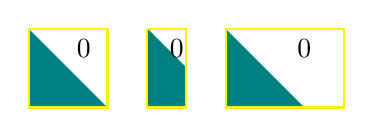
\begin{tikzpicture}[scale=1, transform shape]
	    \tikzset{>=latex}
	    \filldraw[color=teal] (0,1) -- (0,0) -- (1,0);
	    \filldraw[color=teal] (1.5,1) -- (2,0.5) -- (2,0) -- (1.5,0);
	    \filldraw[color=teal] (2.5,1) -- (2.5,0) -- (3.5,0);
	    \draw[color=yellow,thick] (0,0) rectangle (1,1);
	    \draw[color=yellow,thick] (1.5,0) rectangle (2,1);
	    \draw[color=yellow,thick] (2.5,0) rectangle (4,1);
	    \node[] (0) at (0.7,0.75) {$0$};
	    \node[] (0) at (1.88,0.75) {$0$};
	    \node[] (0) at (3.5,0.75) {$0$};
	\end{tikzpicture}
    \end{center}
\end{definition}
}
%-------------- end slide -------------------------------%}}}

%-------------- start slide -------------------------------%{{{ 4
\frame{
\begin{emptytitle}{}
    An \alert{LU factorization} of a matrix $A$ is written
    \begin{align*}
	A = LU
    \end{align*}
    where $L$ is lower triangular matrix and $U$ is upper triangular.
\end{emptytitle}
\bigskip
\pause
\begin{emptytitle}
    We often require either $L$ or $U$ to have only 1's  on the main diagonal.
\end{emptytitle}
\pause
\bigskip
\begin{align*}
    A=
    \begin{pmatrix}
	\textcolor{red}{1}      & 0                       & \cdots                  & 0 \\
	\textcolor{red}{*}      & \textcolor{red}{1}      & \ddots                  & \vdots \\
	\textcolor{red}{\vdots} & \textcolor{red}{\ddots} & \textcolor{red}{\ddots} & 0 \\
	\textcolor{red}{*}      & \textcolor{red}{\cdots} & \textcolor{red}{*}      & \textcolor{red}{1}
    \end{pmatrix}
    \begin{pmatrix}
	\textcolor{red}{*} & \textcolor{red}{*} & \textcolor{red}{\cdots} & \textcolor{red}{*} \\
	0                  & \textcolor{red}{*} & \textcolor{red}{\ddots} & \textcolor{red}{\vdots} \\
	\vdots             & \ddots             & \textcolor{red}{\ddots} & \textcolor{red}{*} \\
	0                  & \cdots             & 0                       & \textcolor{red}{*}
    \end{pmatrix}
\end{align*}
}
%-------------- end slide -------------------------------%}}}

\section[\textcolor{yellow}{}]{\textcolor{yellow}{Why do we need LU Factorization?}}

%-------------- start slide -------------------------------%{{{ 5
\frame{
\frametitle{Why do we need LU Factorization?}
\pause
\begin{emptytitle}
    The $LU$ factorization often helps to quickly  solve equations of the form $A \vec{x} =\vec{b} $.
\end{emptytitle}
\bigskip
\pause
\begin{emptytitle}
    Suppose we wish to find all solutions $\vec{x}$ to the system $A \vec{x} =B$. The $LU$ factorization of $A$ can assist in this process.
    \pause
    \medskip

    Consider the following reduction:
    \begin{eqnarray*}
	A\vec{x}     & = & B \\
	(LU) \vec{x} & = & B \\
	L (U\vec{x}) & = & B \\
	L\vec{y}     & = & B
    \end{eqnarray*}
    \pause
    \medskip

    Therefore, if we can solve $L\vec{y} = B$ for $\vec{y}$, then all that remains is to solve $U\vec{x} = \vec{y}$ for $\vec{x}$.
\end{emptytitle}
}
%-------------- end slide -------------------------------%}}}

%-------------- start slide -------------------------------%{{{ 6
\frame{
\begin{example}
Find all solutions to
\begin{align*}
\leftB \begin{array}{rrrr}
1 & 3 & 2 & 0 \\
3 & 10 & 5 & 1 \\
0 & -1 & 2 & 1
\end{array} \rightB \leftB \begin{array}{c}
x_1 \\
x_2 \\
x_3 \\
x_4
\end{array}
\rightB
 =
\leftB \begin{array}{c}
2 \\
4 \\
6
\end{array}
\rightB
\end{align*}
\end{example}

\pause

\begin{solution}
Using a method of your choice, verify that the $LU$ factorization of $A$ gives
\begin{align*}
L = \leftB \begin{array}{rrr}
1 & 0 & 0 \\
3 & 1 & 0 \\
0 & -1 & 1
\end{array}\rightB, U = \leftB \begin{array}{rrrr}
1 & 3 & 2 & 0 \\
0 & 1 & -1 & 1 \\
0 & 0 & 1 & 2
\end{array} \rightB
\end{align*}

\end{solution}
}
%-------------- end slide -------------------------------%}}}

%-------------- start slide -------------------------------%{{{ 7
\frame{
\begin{solution}[continued]
Let $\vec{y}  = \leftB \begin{array}{c}
y_1 \\
y_2 \\
y_3
\end{array}\rightB$ and solve $L \vec{y}  = \vec{b} $.

\pause

\begin{align*}
\leftB \begin{array}{rrr}
1 & 0 & 0 \\
3 & 1 & 0 \\
0 & -1 & 1
\end{array}\rightB  \leftB \begin{array}{c}
y_1 \\
y_2 \\
y_3
\end{array}\rightB = \leftB \begin{array}{c}
2 \\
4 \\
6
\end{array}
\rightB
\end{align*}

\pause

The solution is $ \vec{y}  = \leftB \begin{array}{r}
2 \\
-2 \\
4
\end{array}\rightB$.

\pause
\medskip

Now we solve $U \vec{x}  = \vec{y} $.
\begin{align*}
\leftB \begin{array}{rrrr}
1 & 3 & 2 & 0 \\
0 & 1 & -1 & 1 \\
0 & 0 & 1 & 2
\end{array} \rightB
 \leftB \begin{array}{c}
x_1 \\
x_2 \\
x_3 \\
x_4
\end{array}
\rightB = \leftB \begin{array}{r}
2 \\
-2 \\
4
\end{array}\rightB
\end{align*}

\end{solution}
}
%-------------- end slide -------------------------------%}}}

%-------------- start slide -------------------------------%{{{ 8
\frame{
\begin{solution}[continued]
    Multiplying and solving (or finding the \rref), the general solution is given by
    \begin{align*}
	\vec{x}  = \leftB \begin{array}{r}
	-12 \\
	2 \\
	4 \\
	0
	\end{array} \rightB
	+
	\leftB \begin{array}{r}
	13 \\
	-3 \\
	-2 \\
	1
	\end{array} \rightB t, \quad \forall t \in \mathbb{R}.
    \end{align*}
    \myQED
\end{solution}
}
%-------------- end slide -------------------------------%}}}

\section[\textcolor{yellow}{}]{\textcolor{yellow}{Finding the LU}}

%-------------- start slide -------------------------------%{{{ 9
\frame{
\frametitle{Finding the LU Factorization}
\pause
\begin{emptytitle}
		\textcolor{yellow}{Condition for the existence of $LU$ factorization:}~ A matrix $A$ has $LU$ factorization provided that $A$ can be \alert{lower reduced}, namely, the \ef of $A$ can be calculated
		without interchanging rows.
\end{emptytitle}
\vfill
\pause
\begin{example}{}
    Determine if the $LU$ factorization of $A$ exists, and if so, find it.
    \begin{align*}
	A = \leftB
	\begin{array}{rrr}
	    1 & 1 & 2 \\
	    2 & 3 & 0 \\
	    1 & 0 & 5
	\end{array}
	\rightB
    \end{align*}
\end{example}
\pause
\vfill
\begin{solution}
    Because the \ef can be obtained without interchanging rows:
    \pause
    \begin{align*}
	\hspace{-3em}
	\leftB
	\begin{array}{rrr}
	    1 & 1 & 2 \\
	    2 & 3 & 0 \\
	    1 & 0 & 5
	\end{array}
	\rightB
	% \onslide<+->
	\xrightarrow{r_2 - 2r_1}
	\leftB
	\begin{array}{rrr}
	    1 & 1 & 2 \\
	    0 & 1 & -4 \\
	    1 & 0 & 5
	\end{array}
	\rightB
	% \onslide<+->
	\xrightarrow{r_3 - r_1}
	\leftB
	\begin{array}{rrr}
	    1 & 1 & 2 \\
	    0 & 1 & -4 \\
	    0 & -1 & 3
	\end{array}
	\rightB
	% \onslide<+->
	\xrightarrow{r_3 + r_2}
	\leftB
	\begin{array}{rrr}
	    1 & 1 & 2 \\
	    0 & 1 & -4 \\
	    0 & 0 & -1
	\end{array}
	\rightB
    \end{align*}
    the LU factorization exists, or $A$ can be lower reduced.
\end{solution}
}
%-------------- end slide -------------------------------%}}}

%-------------- start slide -------------------------------%{{{ 10
\frame{
\begin{solution}[continued]
    We proceed to finding $L$ and $U$. Assign variables to the unknown entries and multiply.
    \begin{eqnarray*}
    A = \leftB
    \begin{array}{rrr}
	1 & 1 & 2 \\
	2 & 3 & 0 \\
	1 & 0 & 5
    \end{array}
    \rightB
    &=& \leftB \begin{array}{ccc}
	1 & 0 & 0 \\
	x & 1 & 0 \\
	y & z & 1
    \end{array} \rightB
    \leftB \begin{array}{ccc}
	a & d & e \\
	0 & b & f \\
	0 & 0 & c
    \end{array} \rightB \\
    &=&
    \leftB \begin{array}{ccc}
	a  & d     & e    \\
	ax & dx+b  & ex+f \\
	ay & dy+bz & ey+fz+c
    \end{array} \rightB
    \end{eqnarray*}
    \pause

    Solving each entry will give us values for the unknown entries.
\end{solution}
}
%-------------- end slide -------------------------------%}}}

%-------------- start slide -------------------------------%{{{ 11
\frame{
\begin{solution}[continued]
    \begin{align*}
	\leftB
	\begin{array}{rrr}
	    1 & 1 & 2 \\
	    2 & 3 & 0 \\
	    1 & 0 & 5
	\end{array}
	\rightB
	 =
	\leftB \begin{array}{ccc}
	    a  & d     & e    \\
	    ax & dx+b  & ex+f \\
	    ay & dy+bz & ey+fz+c
	\end{array} \rightB
    \end{align*}

    \pause

    We see easily that $a = 1, d = 1$, and $e = 2$.  Continuing to solve the first column gives $x = 2, y=1$. The other values are calculated as follows.
    \pause
    \vspace{-2.5em}
    \begin{multicols}{2}
    \begin{eqnarray*}
	dx + b     & = & 3 \\
	(1)(2) + b & = & 3 \\
	b          & = & 1
    \end{eqnarray*}

    \begin{eqnarray*}
	dy + bz       & = & 0 \\
	(1)(1) + (1)z & = & 0 \\
	z             & = & -1
    \end{eqnarray*}

    \columnbreak

    \begin{eqnarray*}
	ex + f     & = & 0 \\
	(2)(2) + f & = & 0 \\
	f          & = & -4
    \end{eqnarray*}

    \begin{eqnarray*}
	ey + fz +c          & = & 5 \\
	(2)(1) + (-4)(-1)+c & = & 5 \\
	c                   & = & -1
    \end{eqnarray*}
    \end{multicols}
\end{solution}
}
%-------------- end slide -------------------------------%}}}

%-------------- start slide -------------------------------%{{{ 12
\frame{
\begin{solution}[continued]
Therefore,

\begin{minipage}{0.48\textwidth}
    \begin{gather*}
       L \\
       | | \\
     \leftB \begin{array}{ccc}
	1 & 0 & 0 \\
	x & 1 & 0 \\
	y & z & 1
    \end{array} \rightB \\
    |  | \\
     \leftB \begin{array}{rrr}
	1 & 0 & 0 \\
	2 & 1 & 0 \\
	1 & -1 & 1
    \end{array} \rightB
    \end{gather*}
\end{minipage}
\pause
\begin{minipage}{0.48\textwidth}
\begin{gather*}
    U \\ || \\
    \leftB \begin{array}{ccc}
	a & d & e \\
	0 & b & f \\
	0 & 0 & c
    \end{array} \rightB
    \\ || \\
    \leftB \begin{array}{rrr}
	1 & 1 & 2 \\
	0 & 1 & -4 \\
	0 & 0 & -1
    \end{array} \rightB
\end{gather*}
\myQED
\end{minipage}
\end{solution}
}
%-------------- end slide -------------------------------%}}}

%-------------- start slide -------------------------------%{{{ 13
\begin{frame}[fragile]
    \begin{remark}
	    If you want the diagonal terms of $U$ to be all $1$'s:
      \bigskip

    \begin{align*}
	 \leftB \begin{array}{rrr}
	    1 & 0 & 0 \\
	    2 & 1 & 0 \\
	    1 & -1 & 1
	\end{array} \rightB
	\textcolor{yellow}{
	\begin{bmatrix}
	    1 & 0 & 0\\
	    0 & 1 & 0\\
	    0 & 0 & -1\\
	\end{bmatrix}
	\begin{bmatrix}
	    1 & 0 & 0\\
	    0 & 1 & 0\\
	    0 & 0 & -1\\
	\end{bmatrix}}
	\leftB \begin{array}{rrr}
	    1 & 1 & 2 \\
	    0 & 1 & -4 \\
	    0 & 0 & -1
	\end{array} \rightB
    \end{align*}
    \begin{align*}
    |  |
    \end{align*}
    \begin{align*}
    \underbrace{
	\leftB \begin{array}{rrr}
	    1 & 0  & \alert{-0} \\
	    2 & 1  & \alert{-0}\\
	    1 & -1 & \alert{-1}
  \end{array} \rightB}_{L}
  \quad
  \underbrace{
	\leftB \begin{array}{rrr}
	    1          & 1          & 2 \\
	    0          & 1          & -4 \\
	    \alert{-0} & \alert{-0} & \alert{1}
	\end{array} \rightB}_{U}
    \end{align*}
    \myQED
\end{remark}

\end{frame}
%-------------- end slide -------------------------------%}}}

\section[\textcolor{yellow}{}]{\textcolor{yellow}{Multiplier Method}}

%-------------- start slide -------------------------------%{{{ 14
\frame{
\frametitle{Multiplier Method}
\pause
\begin{emptytitle}
    The following process for finding $L$ and $U$, called the \alert{multiplier method}, can be more efficient.
\end{emptytitle}
\pause
\vfill
\begin{example}
    Find the $LU$ factorization of $A = \leftB
    \begin{array}{rrr}
	1 & 1 & 2 \\
	2 & 3 & 0 \\
	1 & 0 & 5
    \end{array}
    \rightB$
\end{example}
\pause
\vfill
\begin{solution}
    First, write $A$ as
    \begin{align*}
    \leftB
    \begin{array}{rrr}
	1 & 1 & 2 \\
	2 & 3 & 0 \\
	1 & 0 & 5
    \end{array}
    \rightB
    \end{align*}
    \begin{align*} || \end{align*}
    \begin{align*}
	\leftB
    \begin{array}{rrr}
	1 & 0 & 0 \\
	0 & 1 & 0 \\
	0 & 0 & 1
    \end{array}
    \rightB\leftB
    \begin{array}{rrr}
	1 & 1 & 2 \\
	2 & 3 & 0 \\
	1 & 0 & 5
    \end{array}
    \rightB
    \end{align*}

    \pause

    Now we will use row operations (except for interchanging rows) to transform the right side into the appropriate $L$ and $U$.
\end{solution}
}
%-------------- end slide -------------------------------%}}}

%-------------- start slide -------------------------------%{{{ 15
\frame{
\begin{solution}[continued]
    To do so, we use row operations to remove the entries of $A$ below the main diagonal. For every operation we apply to $A$ (the matrix on the right), we apply the inverse operation to the identity matrix (on the left). This ensures the product remains the same.

    \pause
    \medskip

    The first step is to add $(-2)$ times the first row of $A$ to the second row.
    To preserve the product, add $(2)$ times the second column to the first column, for the matrix on the left.
    \begin{align*}||\end{align*}
    \begin{align*}
	    \leftB
	\begin{array}{rrr}
	    1 & 0 & 0 \\
	    0 & 1 & 0 \\
	    0 & 0 & 1
	\end{array}
	\rightB
	\textcolor{yellow}{
	\begin{bmatrix}
	    1 & 0 & 0\\
	    2 & 1 & 0\\
	    0 & 0 & 1\\
	\end{bmatrix}}
	\textcolor{green}{
	\begin{bmatrix}
	    1  & 0 & 0 \\
	    -2 & 1 & 0 \\
	    0  & 0 & 1 \\
	\end{bmatrix}}
	\leftB
	\begin{array}{rrr}
	    1 & 1 & 2 \\
	    2 & 3 & 0 \\
	    1 & 0 & 5
	\end{array}
	\rightB
    \end{align*}
    \begin{align*}||\end{align*}
    \begin{align*}
	c_1 + 2c_2 \to c_1\;
	\leftB
	\begin{array}{rrr}
	    1 & 0 & 0 \\
	    2 & 1 & 0 \\
	    0 & 0 & 1
	\end{array}
	\rightB\leftB
	\begin{array}{rrr}
	    1 & 1 & 2 \\
	    0 & 1 & -4 \\
	    1 & 0 & 5
	\end{array}
	\rightB
	\; r_2 - 2r_1 \to r_2
    \end{align*}
\end{solution}
}
%-------------- end slide -------------------------------%}}}

%-------------- start slide -------------------------------%{{{ 16
\frame{
\begin{solution}[continued]
    We proceed in the same way.

    \begin{align*}
    c_1 + c_3 \to c_1 \;
    \leftB
    \begin{array}{rrr}
	1 & 0 & 0 \\
	2 & 1 & 0 \\
	1 & 0 & 1
    \end{array}
    \rightB\leftB
    \begin{array}{rrr}
	1 & 1 & 2 \\
	0 & 1 & -4 \\
	0 & -1 & 3
    \end{array}
    \rightB
    \; r_3 - r_1 \to r_3
    \end{align*}

    \pause
    \begin{align*}
    c_2 - c_3 \to c_2
    \leftB
    \begin{array}{rrr}
	1 & 0  & 0 \\
	2 & 1  & 0 \\
	1 & -1 & 1
    \end{array}
    \rightB\leftB
    \begin{array}{rrr}
	1 & 1 & 2 \\
	0 & 1 & -4 \\
	0 & 0 & -1
    \end{array}
    \rightB
    \; r_3 + r_2 \to r_3
    \end{align*}

    \bigskip
    \pause

    At this point we have a lower triangular matrix $L$ on the left, and an upper triangular matrix $U$ on the right so we are done. You can (and should!) check that this product equals $A$.
    \bigskip

    If you want the diagonal terms of $U$ to be all $1$'s:
    \begin{align*}
    -1\times c_3 \to c_3
    \leftB
    \begin{array}{rrr}
	1 & 0  & 0 \\
	2 & 1  & 0 \\
	1 & -1 & -1
    \end{array}
    \rightB\leftB
    \begin{array}{rrr}
	1 & 1 & 2 \\
	0 & 1 & -4 \\
	0 & 0 & 1
    \end{array}
    \rightB
    \; -1\times r_3 \to r_3
    \end{align*}
    \myQED
\end{solution}
}
%-------------- end slide -------------------------------%}}}

%-------------- start slide -------------------------------%{{{ 17
\frame{
\begin{problem}
    Use the multiplier method to verify the $LU$ factorization for
    \begin{align*}
	A = \leftB \begin{array}{rrr}
	    1  & 4  & 2 \\
	    3  & 13 & 5 \\
	    -2 & -7 & -4
	\end{array} \rightB
    \end{align*}
\end{problem}
\pause
\vfill
\begin{solution}
    \begin{align*}
	A = \leftB \begin{array}{rrr}
	    1  & 4  & 2 \\
	    3  & 13 & 5 \\
	    -2 & -7 & -4
	\end{array} \rightB = \leftB \begin{array}{rrr}
	    1  & 0 & 0 \\
	    3  & 1 & 0 \\
	    -2 & 1 & 1
	\end{array} \rightB
	\leftB \begin{array}{rrr}
	    1 & 4 & 2 \\
	    0 & 1 & -1 \\
	    0 & 0 & 1
	\end{array} \rightB = LU
    \end{align*}
    \myQED
\end{solution}
}
%-------------- end slide -------------------------------%}}}

\section[\textcolor{yellow}{}]{\textcolor{yellow}{LU-Algorithm}}
%-------------- start slide -------------------------------%{{{ 1
\begin{frame}[fragile]
\begin{theorem}[ LU-Algorithm ] % {{{
Let $A$ be an $m \times n$ matrix of $\func{rank }r$, and suppose that $A$ can
be lower reduced to a row-echelon matrix $U$. Then $A = LU$ where the lower
triangular, invertible matrix $L$ is constructed as
follows:

\begin{enumerate}
\item If $A = 0$, take $L = I_{m}$ and $U = 0$.
\item If $A \neq 0$, write $A_{1} = A$ and let $\vec{c}_{1}$ be the
    \textcolor{yellow}{leading column} of $A_{1}$. Use $\vec{c}_{1}$ to create
    the first leading $1$ and make its below all zeros. When this is completed,
    let $A_{2}$ denote the matrix consisting of rows 2 to $m$ of the matrix
    just created.
\item If $A_{2} \neq 0$, let $\vec{c}_{2}$ be the leading column of $A_{2}$ and
    repeat Step 2 on $A_{2}$ to create $A_{3}$.
\item Continue in this way until $U$ is reached, where all rows below the last
    leading $1$ consist of zeros. This will happen after $r$ steps.
\item Create $L$ by placing $\vec{c}_{1}, \vec{c}_{2}, \dots, \vec{c}_{r}$ at
    the bottom of the first $r$ columns of $I_{m}$.
\end{enumerate}
\end{theorem} % }}}
\end{frame}
%-------------- end slide -------------------------------%}}}
%-------------- start slide -------------------------------%{{{ 1
\begin{frame}[fragile]
\begin{problem} %{{{
Find an LU-factorization for $A = \leftB \begin{array}{rrr}
2 & 4 & 2 \\
1 & 1 & 2 \\
-1 & 0 & 2
\end{array} \rightB$.
\end{problem} % }}}

\begin{solution}
\begin{equation*}
\leftB \begin{array}{rrr}
    \tn{exa4a}{\textcolor{yellow}{2}}  & 4 & 2 \\
    \textcolor{yellow}{1}              & 1 & 2 \\
    \tn{exa4b}{\textcolor{yellow}{-1}} & 0 & 2
\end{array} \rightB \rightarrow
\leftB \begin{array}{rrr}
    1 & 2                                & 1 \\
    0 & \tn{exa4c}{\textcolor{blue}{-1}} & 1 \\
    0 & \tn{exa4d}{\textcolor{blue}{2}}  & 3
\end{array} \rightB \rightarrow
\leftB \begin{array}{rrr}
    1 & 2 & 1  \\
    0 & 1 & -1 \\
    0 & 0 & \tn{exa4e}{\alert{5}}
\end{array} \rightB \rightarrow
\leftB \begin{array}{rrr}
    1 & 2 & 1 \\
    0 & 1 & -1 \\
    0 & 0 & 1
\end{array} \rightB = U
\end{equation*}
\pause
\begin{tikzpicture}[remember picture, overlay]
\draw[color=blue!30!gray,rounded corners]([xshift=-12pt, yshift=5pt]exa4a.north west) rectangle ([xshift=5pt, yshift=-5pt]exa4b.south east);
\draw[color=blue!30!gray,rounded corners]([xshift=-4pt, yshift=5pt]exa4c.north west) rectangle ([xshift=5pt, yshift=-5pt]exa4d.south east);
\draw[color=blue!30!gray,rounded corners]([xshift=-4pt, yshift=5pt]exa4e.north west) rectangle ([xshift=4pt, yshift=-5pt]exa4e.south east);
\end{tikzpicture}
\hspace{-2em}
\begin{equation*}
\leftB \begin{array}{rrr}
    1 & 0 & 0 \\
    0 & 1 & 0 \\
    0 & 0 & 1
\end{array} \rightB \rightarrow
\leftB \begin{array}{rrr}
    \textcolor{yellow}{2}  & 0 & 0 \\
    \textcolor{yellow}{1}  & 1 & 0 \\
    \textcolor{yellow}{-1} & 0 & 1
\end{array} \rightB \rightarrow
\leftB \begin{array}{rrr}
    \textcolor{yellow}{2}  & 0                    & 0 \\
    \textcolor{yellow}{1}  & \textcolor{blue}{-1} & 0 \\
    \textcolor{yellow}{-1} & \textcolor{blue}{2}  & 1
\end{array} \rightB \rightarrow
\leftB \begin{array}{rrr}
    \textcolor{yellow}{2}  & 0                    & 0 \\
    \textcolor{yellow}{1}  & \textcolor{blue}{-1} & 0 \\
    \textcolor{yellow}{-1} & \textcolor{blue}{2}  &\alert{5}
\end{array} \rightB
= L
\end{equation*}
% \[\Downarrow\]
% \begin{align*}
%   L = \leftB \begin{array}{rrr}
%       \textcolor{yellow}{2}  & 0                    & 0 \\
%       \textcolor{yellow}{1}  & \textcolor{blue}{-1} & 0 \\
%       \textcolor{yellow}{-1} & \textcolor{blue}{2}  & \alert{5}
% \end{array} \rightB
% \end{align*}
\myQED
\end{solution}
\end{frame}
%-------------- end slide -------------------------------%}}}
%-------------- start slide -------------------------------%{{{ 1
\begin{frame}[fragile]

\begin{problem} %{{{
Find an LU-factorization for $A = \leftB \begin{array}{rrrrr}
5 & -5 & 10 & 0 & 5 \\
-3 & 3 & 2 & 2 & 1 \\
-2 & 2 & 0 & -1 & 0 \\
1 & -1 & 10 & 2 & 5
\end{array} \rightB$.
\end{problem} % }}}
\end{frame}
%-------------- end slide -------------------------------%}}}
%-------------- start slide -------------------------------%{{{ 1
\begin{frame}[fragile]
\begin{solution}
    \begin{minipage}{0.45\textwidth}
        \begin{gather*}
        \leftB \begin{array}{rrrrr}
            \tn{exa3a}{\textcolor{yellow}{5}} & -5 & 10 & 0  & 5 \\
            \textcolor{yellow}{-3}            & 3  & 2  & 2  & 1 \\
            \textcolor{yellow}{-2}            & 2  & 0  & -1 & 0 \\
            \tn{exa3b}{\textcolor{yellow}{1}} & -1 & 10 & 2  & 5
        \end{array} \rightB \\
        \downarrow\\
        \leftB \begin{array}{rrrrr}
            1 & -1 & 2                               & 0  & 1 \\
            0 & 0  & \tn{exa3c}{\textcolor{blue}{8}} & 2  & 4 \\
            0 & 0  & \textcolor{blue}{4}             & -1 & 2 \\
            0 & 0  & \tn{exa3d}{\textcolor{blue}{8}} & 2  & 4
        \end{array} \rightB \\
        \downarrow\\
        \leftB \def\arraystretch{1.5}\begin{array}{rrrrr}
            1 & -1 & 2 & 0                      & 1   \\
            0 & 0  & 1 & 1/4                    & 1/2 \\
            0 & 0  & 0 & \tn{exa3e}{\alert{-2}} & 0   \\
            0 & 0  & 0 & \tn{exa3f}{\alert{0}}  & 0
        \end{array} \rightB\\
        \downarrow
        \end{gather*}
    \end{minipage}
    \begin{minipage}{0.45\textwidth}
        \begin{gather*}
        \leftB \def\arraystretch{1.5}\begin{array}{rrrrr}
            1 & -1 & 2 & 0   & 1   \\
            0 & 0  & 1 & 1/4 & 1/2 \\
            0 & 0  & 0 & 1   & 0   \\
            0 & 0  & 0 & 0   & 0
        \end{array} \rightB\\
        || \\
        U
        \end{gather*}
        \pause
        \[\Downarrow\]
    \begin{gather*}
        L \\
        ||\\
    \leftB \begin{array}{rrrrr}
        \textcolor{yellow}{5}  & 0                   & 0          & 0 \\
        \textcolor{yellow}{-3} & \textcolor{blue}{8} & 0          & 0 \\
        \textcolor{yellow}{-2} & \textcolor{blue}{4} & \alert{-2} & 0 \\
        \textcolor{yellow}{1}  & \textcolor{blue}{8} & \alert{0}  & 1
    \end{array} \rightB
    \end{gather*}
    \myQED
    \end{minipage}
\begin{tikzpicture}[remember picture, overlay]
\draw[color=blue!30!gray,rounded corners]([xshift=-12pt, yshift=5pt]exa3a.north west) rectangle ([xshift=5pt, yshift=-5pt]exa3b.south east);
\draw[color=blue!30!gray,rounded corners]([xshift=-7pt, yshift=5pt]exa3c.north west) rectangle ([xshift=5pt, yshift=-5pt]exa3d.south east);
\draw[color=blue!30!gray,rounded corners]([xshift=-4pt, yshift=5pt]exa3e.north west) rectangle ([xshift=5pt, yshift=-5pt]exa3f.south east);
\end{tikzpicture}

\end{solution}
\end{frame}
%-------------- end slide -------------------------------%}}}
\end{document}
